\documentclass{article}
\usepackage[utf8]{inputenc}
\usepackage[T2A]{fontenc}
\usepackage[utf8]{inputenc}
\usepackage{float}
%\usepackage[russian]{babel}
\usepackage[a4paper, left=10mm, right=10mm, top=20mm, bottom=20mm]{geometry}
\usepackage{natbib}
\usepackage{graphicx}
\usepackage{tabularx}
\usepackage{hyperref}

\title{PSD@CBM firmware description (draft, for internal use)}
\author{Finogeev Dmitry, INR RAS}





\begin{document}

\maketitle

Actual version of the document is avaliable at github:
\newline
\url{https://github.com/dfinogee/PSD-readout-manual/raw/main/PSD_readout_manual.pdf}



\tableofcontents

\newpage

\section{ADC data processing}

\subsection{Channel data collecting}
Each channel collect data in FIFO (chdata\_fifo) in hit packet format and emit ready signal after data stored in fifo. Ready signal is synchronous to signal threshold crossing and used for event ADC timestamp fig.~\ref{fig:1}. It is implemented in PSD\_channel\_calc.

\begin{figure}[H]
	\centering 
	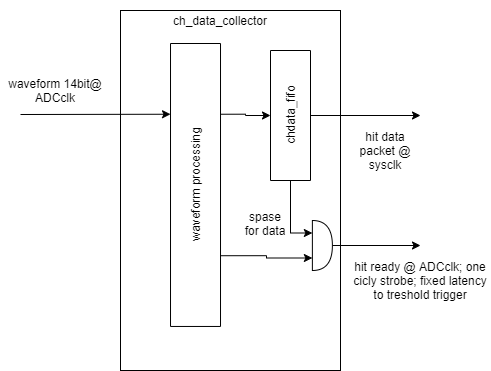
\includegraphics[width=0.5\textwidth]{ADC_event_collection.png}
	\caption{\label{fig:1} Channel data collecting scheme}
\end{figure}
Mean hit rate per channel = SYSCKL / total channels + 2 sys cycle / packet length. SYSCKL = n * ADCclk = 240MHz; total channels = 32; packet lenght = 1. Max mean hit rate is 7 MHz. (0.78 MHz with 80MHz and 2 waveform packets; 2.2 for 10 channels)


Hit packet forming is implemented in ch\_data\_colletcor with three fifos. raw\_waveform\_fifo write raw ADC data by wf\_strobe signal. header\_ch\_fifo store zero level (if future all data avaliable at the beginning of waveform calculation) by strobe start signal. calc\_ready signal raised for one cycle when charge (fit in future) is ready. By calc\_ready signal hit header with charge and data from header\_ch\_fifo is written to chdata\_fifo, header\_ch\_fifo is readed, counter started to read raw\_waveform\_fifo. fig.~\ref{fig:2} Represents forming hit packet.

todo: data with out raw data
todo: ch ready signal after packet pushed
todo: readout rate, missing packets

\begin{figure}[H]
	\centering 
	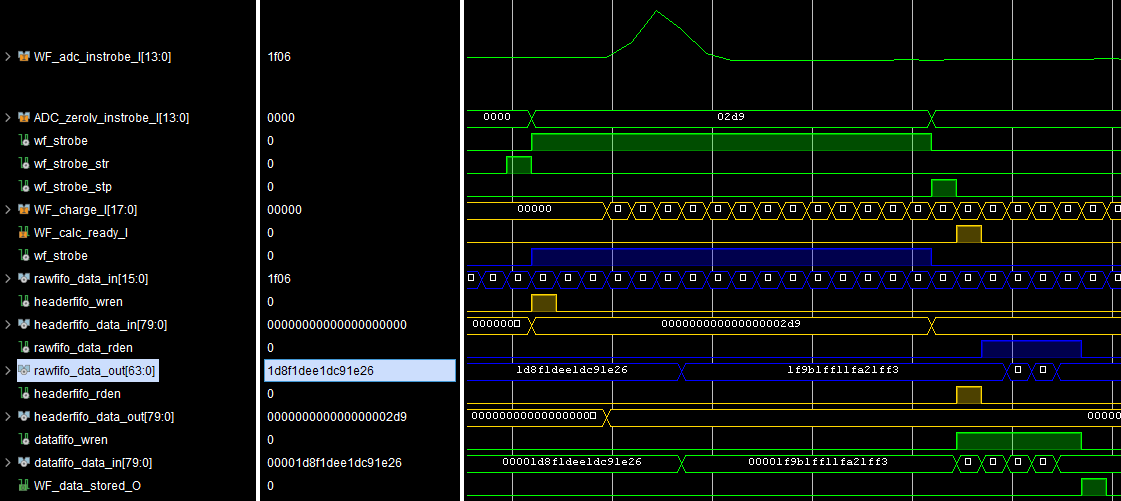
\includegraphics[width=1.0\textwidth]{ADC_ch_data_collector_wave.png}
	\caption{\label{fig:2} Channel data collecting signals}
\end{figure}





\begin{table}[H]
\centering
\begin{tabular}{| l | l | l | l | l | l |}
\hline
word & 79 .. 72 & 71 .. 64 & 63 .. 34 & 33 .. 16 & 15 .. 0 \\ \hline
1 & num data words & channel & 0x0 & signal charge & waveform zero level \\ \hline
\end{tabular}
\caption{hit packet header.\label{tab1}}
\end{table}

\begin{table}[H]
\centering
\begin{tabular}{| l | l | l | l | l | l |}
\hline
word & 79 .. 64 & 63 .. 48 & 47 .. 32 & 31 .. 16 & 15 .. 0 \\ \hline
1 & 0x0 & waveform point n & waveform point n+1 & waveform point n+2 & waveform point n+3 \\ \hline
\end{tabular}
\caption{hit packet data word.\label{tab1}}
\end{table}








\subsection{Data collecting from channels fifo}

Each channel generate single strobe with fixed latency to threshold crossing indicating waveform measurement. 32 bit strobe word is trored to data\_wf\_calc\_fifo with mc index and ADC timestamp. FSM read stored strobes and collect data from fired channels storing outputs to common\_data\_fifo, each event header word with timing and size info stored in common\_header\_fifo. Shematic represented on figure ~\ref{fig:3}.

\begin{figure}[H]
	\centering 
	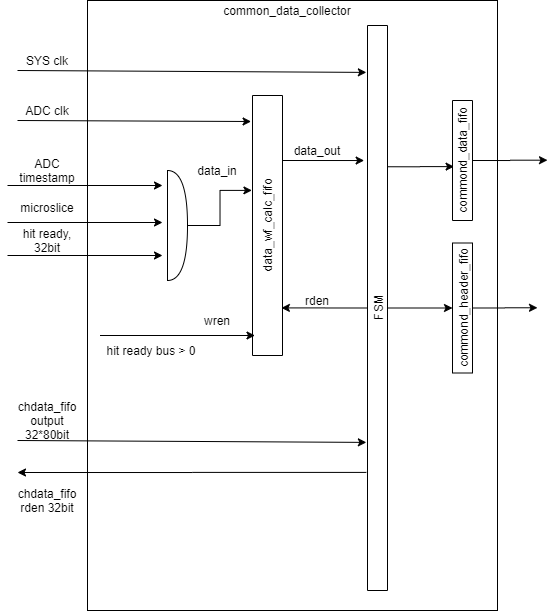
\includegraphics[width=0.5\textwidth]{ADC_common_event_collection.png}
	\caption{\label{fig:3} Data collecting scheme from all channels fifos}
\end{figure}


FSM is switched from wait to start state when data\_wf\_calc\_fifo\_isempty became '0' and fifo output is latched. Priority encoder show next fired channel from strobe and data collected from fired channel to common\_data\_fifo with hit\_packet\_iterator. input to priory encoder is shifted to bit after fired channel when iterator reach last number. Priority encoder could be equal or less than 32 bit. Simulation outputs presented on figure ~\ref{fig:4}.

\begin{figure}[H]
	\centering 
	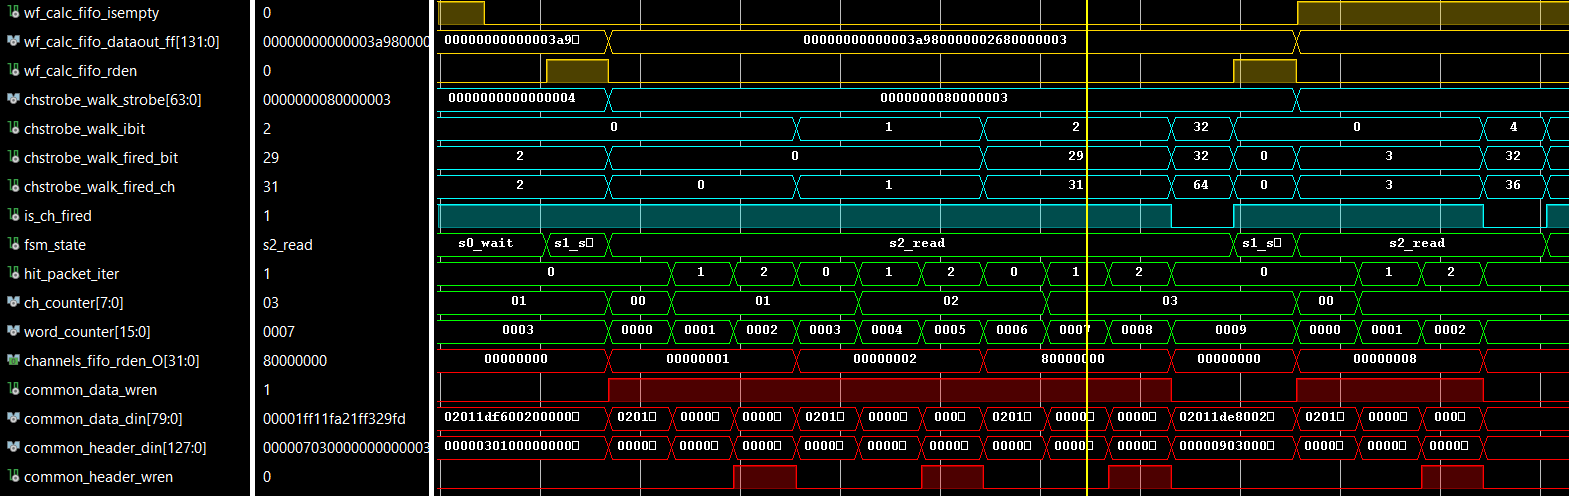
\includegraphics[width=1.0\textwidth]{ADC_common_data_collector_wave.png}
	\caption{\label{fig:4} Data collecting signal from all channels fifos}
\end{figure}







todo: waveform bias
todo: data without waveforms
todo: reset wignal for data and sys clocks.
todo: readout rate, missing packets

\section{ADC control}
\subsection{control registers}

\begin{table}[H]
\centering
\begin{tabular}{| l | l | l | l | l | l | l | l | l | l | l |}
\hline
addr & 31 .. 30 & 29 .. 28 & 27 .. 24 & 23 .. 20 & 19 .. 16 & 15 .. 14 & 13 .. 12 & 11 .. 8 & 7 .. 4 & 3 .. 0 \\ \hline
0 & 0x0 & \multicolumn{4}{c|}{threshold ch1} & 0x0 & \multicolumn{4}{c|}{threshold ch0} \\ \hline
1 & 0x0 & \multicolumn{4}{c|}{threshold ch3} & 0x0 & \multicolumn{4}{c|}{threshold ch2} \\ \hline
2 & 0x0 & \multicolumn{4}{c|}{threshold ch5} & 0x0 & \multicolumn{4}{c|}{threshold ch4} \\ \hline
3 & 0x0 & \multicolumn{4}{c|}{threshold ch7} & 0x0 & \multicolumn{4}{c|}{threshold ch6} \\ \hline
4 & 0x0 & \multicolumn{4}{c|}{threshold ch9} & 0x0 & \multicolumn{4}{c|}{threshold ch8} \\ \hline
5 & 0x0 & \multicolumn{4}{c|}{threshold ch11} & 0x0 & \multicolumn{4}{c|}{threshold ch10} \\ \hline
6 & 0x0 & \multicolumn{4}{c|}{threshold ch13} & 0x0 & \multicolumn{4}{c|}{threshold ch12} \\ \hline
7 & 0x0 & \multicolumn{4}{c|}{threshold ch15} & 0x0 & \multicolumn{4}{c|}{threshold ch14} \\ \hline
8 & 0x0 & \multicolumn{4}{c|}{threshold ch17} & 0x0 & \multicolumn{4}{c|}{threshold ch16} \\ \hline
9 & 0x0 & \multicolumn{4}{c|}{threshold ch19} & 0x0 & \multicolumn{4}{c|}{threshold ch18} \\ \hline
10 & 0x0 & \multicolumn{4}{c|}{threshold ch21} & 0x0 & \multicolumn{4}{c|}{threshold ch20} \\ \hline
11 & 0x0 & \multicolumn{4}{c|}{threshold ch23} & 0x0 & \multicolumn{4}{c|}{threshold ch22} \\ \hline
12 & 0x0 & \multicolumn{4}{c|}{threshold ch25} & 0x0 & \multicolumn{4}{c|}{threshold ch24} \\ \hline
13 & 0x0 & \multicolumn{4}{c|}{threshold ch27} & 0x0 & \multicolumn{4}{c|}{threshold ch26} \\ \hline
14 & 0x0 & \multicolumn{4}{c|}{threshold ch29} & 0x0 & \multicolumn{4}{c|}{threshold ch28} \\ \hline
15 & 0x0 & \multicolumn{4}{c|}{threshold ch31} & 0x0 & \multicolumn{4}{c|}{threshold ch30} \\ \hline
\end{tabular}
\caption{ADC channels threshold control.\label{tab2}}
\end{table}

\begin{table}[H]
\centering
\begin{tabular}{| l | l | l | l | l | l | l | l | l |}
\hline
addr & 31 .. 28 & 27 .. 24 & 23 .. 20 & 19 .. 16 & 15 .. 12 & 11 .. 8 & 7 .. 4 & 3 .. 0 \\ \hline
16 & \multicolumn{4}{c|}{0x0} & waveform length 0..3 [(reg+1)*4] & strobe offset 0..12 & \multicolumn{2}{c|}{control bits} \\ \hline
17 & \multicolumn{8}{c|}{negative channel mask ibit = ich} \\ \hline
\end{tabular}
\caption{ADC readout control.\label{tab3}}
\end{table}

\begin{table}[H]
\centering
\begin{tabular}{| l | l |}
\hline
bit & description \\ \hline
0 & send waveform \\ \hline
1 & ms gen standalone \\ \hline
2 & readout fsm reset \\ \hline
3 & errors reset \\ \hline
\end{tabular}
\caption{Control bits\label{tab4}}
\end{table}


\begin{table}[H]
\centering
\begin{tabular}{| l | l | l | l | l | l | l | l | l |}
\hline
addr & 31 .. 18 & 17 .. 17 & 16 .. 16 & 15 .. 8 & 7 .. 7 & 6 .. 0 \\ \hline
18 & 0x0 & WR & ENA & DATA & 0x0 & ADDR \\ \hline
\end{tabular}
\caption{HV control via I2C.\label{tab5}}
\end{table}

\end{document}

